\documentclass{article}
\usepackage{amsmath, amsthm, amssymb, wasysym, verbatim, color, graphics, geometry, systeme}
\usepackage[]{hyperref}
\usepackage{tikz}

\usepackage{mathrsfs,scalerel}
\newsavebox\foobox
\newlength{\foodim}
\newcommand{\slantbox}[2][0]{\mbox{%
        \sbox{\foobox}{#2}%
        \foodim=#1\wd\foobox
        \hskip \wd\foobox
        \hskip -0.5\foodim
        \pdfsave
        \pdfsetmatrix{1 0 #1 1}%
        \llap{\usebox{\foobox}}%
        \pdfrestore
        \hskip 0.5\foodim
}}
\def\Laplace{\ThisStyle{\slantbox[-.45]{$\SavedStyle\mathscr{L}$}}}

\geometry{tmargin=.75in, bmargin=.75in, lmargin=.75in, rmargin = .75in}  

\newcommand{\R}{\mathbb{R}}
\newcommand{\C}{\mathbb{C}}
\newcommand{\Z}{\mathbb{Z}}
\newcommand{\N}{\mathbb{N}}
\newcommand{\Q}{\mathbb{Q}}
\newcommand{\Cdot}{\boldsymbol{\cdot}}

\newtheorem{thm}{Theorem}
\newtheorem{defn}{Definition}
\newtheorem{conv}{Convention}
\newtheorem{rem}{Remark}
\newtheorem{lem}{Lemma}
\newtheorem{cor}{Corollary}

\theoremstyle{definition}
\newtheorem{example}{Example}[section]

\title{Running Lecture Outline: 707}
\author{[Chirayu Salgarkar]}
\date{Fall 2024}

\begin{document}

\maketitle
\tableofcontents

\vspace{.25in}
\section{26-AUG-24}
\subsection{Order, Linear, and PDE vs ODE}
Not notated. Will add when I have time. 
\section{28-AUG-24}

\subsection{Miscellaneous}
Prof is Phillip Hutton. There are several ways to take the quiz. Quiz, office hours, etc. you can also take it in class. All quiz get one page cheat sheet. 

\subsection{Verifying solutions using initial conditions}
To verify potential solutions, plug into the original diffeq. Use algebra (ha!) to make LHS = RHS. On the other hand, we can simply plug in various numbers for $x$ and check for equivalency. Obviously, check for domains. 
\begin{example}
   \[ y' = xy^{\frac{1}{2}}\]
Potential Solution: \[y = \frac{1}{16}x^4\]
Then, 
    \[\frac{dy}{dx} = \frac{1}{4}x^3 \]
Then, plug into the original diffeq. We have:
    \[ \frac{1}{4}x^3 = x \cdot (\frac{1}{16}x^4)^{\frac{1}{2}}\]
or that
    \[\frac{1}{4}x^3 = \frac{1}{4}x^3 \]
as desired. 
\end{example}

\begin{example}
    \[ (y-x)\frac{dy}{dx} = y-x+8\]
     Potential Solution 1: \[y = 2x + 4\sqrt{x+2}\]
    Potential Solution 2: \[y = x + 4\sqrt{x+2}\]
    Case 1:
     \[\frac{dy}{dx} = 2 + 2(x+2)^{\frac{-1}{2}} \]
     Then, plug into the original diffeq. We have:
     \[ (2x + 4\sqrt{x+2} - x)(2 + 2(x+2)^{\frac{-1}{2}}) = 2x + 4\sqrt{x+2} -x+8\]
     Simplifying,
    \[ (x + 4\sqrt{x+2})(2 + 2(x+2)^{\frac{-1}{2}}) = x+8 + 4\sqrt{x+2}\]
    Consider the case that $x=0$. Then,
    \[ (4\sqrt{2})(2 + 2(2)^{\frac{-1}{2}}) = 8 + 4\sqrt{2}\]
    \[8\sqrt{2} + 8 = 8 + 4\sqrt{2} \] 
    or that 
    \[8\sqrt{2} = 4\sqrt{2}\] 
 which is clearly false. 

 Solution 2 works. You plug it in like above, but end with a true statement. 
 \end{example}
 \subsection{IVPs}
 Solving a diffeq yields a \textit{general} solution with unknowns. Using initial values we can then solve for said unknowns. For $n$ unknowns, we need $n$ initial values. 

 Let's do an example!
 \begin{example}
    $y' = y$, where $y(0) = 3$.
    We know our general solution is 
    \[y = Ce^x\]
    but what is $C$?
    clearly, since $y(0) = 3$, and at $x = 0$, $y=c$, $3 = C$. Thus, the equation is really 
    \[y = 3e^x\]
 \end{example}
 \begin{example}
    $y' + 2xy^2 = 0$, where $y(0)=1$.
    The general solution to this is $y = \frac{1}{x+C}$. Plugging in at $x=0$, we have $C=-1$. Final solution is $y = \frac{1}{x-1}$.
 \end{example}
 \begin{example}
    $x'' + 16x = 0$, where $x(\frac{\pi}{2})= -2$, $x'(\frac{\pi}{2}) = 1$. The general solution is 
    \[x = C_1\cos{4t}+C_2\sin{4t}\]

    You plug in twice, you get $C_1 = -2$ and after the second step you get $C_2 = \frac{1}{4}$. Then plug in to general equation. Yay.
\end{example}
\section{30-AUG-24}
\subsection{Integrating Factor}
This is the most fun McIlwain review. When do we use this?
\begin{thm}
    If you can write a differential equation to be of the form $\frac{dy}{dx} + p(x)y = f(x)$, you are eligible to use Integrating Factor.
\end{thm}

The algorithm for solving goes something like this:
\[
\frac{dy}{dx} + p(x)y = f(x)
\]
Multiply both sides by:
\[
I_f = e^{\int{p(x) \, dx}}
\]
You get:
\[
e^{\int{p(x) \, dx}} \frac{dy}{dx} + e^{\int{p(x) \, dx}} p(x) y = e^{\int{p(x) \, dx}} f(x)
\]
Using reverse chain rule:
\[
\frac{d}{dx}[e^{\int{p(x) \, dx}}y]= e^{\int{p(x) \, dx}} f(x)
\]
Integrating both sides, we get:
\[
    e^{\int{p(x) \, dx}}y = \int{e^{\int{p(x) \, dx}} f(x)}
\]

This gets us:
\[y(x) = \frac{\int{e^{\int{p(x) \, dx}} f(x)}}{e^{\int{p(x) \, dx}}}\]

\begin{example}
    \[\frac{dy}{dx} = 5y\]
This seems separable, and it is. But if you were to use integrating factor, it goes like this:
\[
    \frac{dy}{dx} - 5y = 0
\]
Note that this makes $p(t) = -5$
\[
y = Ce^{5x}
\]
\end{example}

\begin{example}
    \[\frac{dy}{dx} + y = e^{3x}\]

Note that this makes $p(x) = 1$, $f(x) = e^{3x}$
\[
e^{x}\frac{dy}{dx} = e^{3x}e^x = e^{4x}
\]
\[
e^{x}y = \frac{1}{4}e^{4x} + C
\]

\[
y = \frac{\frac{1}{4}e^{4x} + C}{e^{x}}
\]
or:
\end{example}
\section{04-SEP-24}
We have a quiz lol. Three questions, about 20-25 minutes. 
\subsection{Separation of Variables}
\begin{defn}[separable]
A differential equation is separable if you can put it into the form  $\frac{dy}{dx} = f(x)h(y)$, where $f$ $h$ are functions. 
\end{defn}
The steps to solving them are as follows:
\[ 
    \frac{dy}{dx} = f(x)h(y)
\]

\[ 
    \frac{dy}{h(y)} = f(x)dx
\]
\[ 
    \int{\frac{dy}{h(y)}} = \int{f(x)dx}
\]
then, solve. 
Let's check for separability of some cases:
\begin{example}
   \[\frac{dy}{dx} - y = \cos{x}\]
   \[\frac{dy}{dx} = \cos{x} + y\]
   This does not satisfy the form specified in the definition, so it is \textit{not separable}.
\end{example}
\begin{example}
    \[\frac{dy}{dx} = x^2y^4e^{5x-3y}\]
    We can rewrite as:
    \[\frac{dy}{dx} = (x^2e^{5x})(y^4e^{-3y})\]
    This is separable, as it satisfies the above form. 
 \end{example}
Now, let's solve one: 
\begin{example}
    \[(1-x)dy = -ydx \]
where $y(0) = 5$

Rewriting, we get:
\[\frac{1}{1-x}dx = \frac{-1}{y}dy \]
Integrating, we get:
\[ - \ln{1-x} = - \ln{y} + C\]
When $y(0) = 5$, we have $0 = - \ln{5} + C$, so $C = \ln{5}$
So, \[ - \ln{1-x} = - \ln{y} + \ln{5}\]
and then:
\[\ln{y} = \ln{1-x} + \ln{5}\] 
Exponentiating, 
\[e^{\ln{y}} = e^{\ln{1-x} + \ln{5}} \]

\[y = 5(1-x) \]
\end{example}

\begin{example}
    \[\frac{1}{y}\frac{dy}{dx} = 1-x\]
    where $y(0) = 2$
The joke is you don't actually need to use separation to do this. But you can. 
\end{example}


\section{06-SEP-24}
\subsection{Exact Equations}
Exact equations are a specific form of differential equation. 
\begin{defn}
For $f(x,y) = k$, where $k$ is a constant, then $df = \frac{df}{dx}dx + \frac{df}{dy}dy = 0$.
\end{defn}

Then, let us define $M(x,y) = \frac{df}{dx}$ and $N(x,y) = \frac{df}{dy}$. So, $M(x,y)dx + N(x,y)dy = 0$. 
Differentiating, we get:
\[\frac{dm}{dy} = \frac{d^2f}{dxdy} = \frac{dN}{dx}\]

\begin{defn}
If $M(x,y)dx + N(x,y)dy = 0$ and $\frac{dm}{dy} = \frac{d^2f}{dxdy} = \frac{dN}{dx}$, then $\frac{df}{dx} = M$ and $\frac{df}{dy} = N$.
\end{defn}

This gives us a general algorithm for solving differential equations of some classes: 
\begin{enumerate}
    \item Put the DE into form $M(x,y)dx + N(x,y)dy = 0$
    \item Then, identify $M(x,y)$ and $N(x,y)$
    \item Then, test for exactness: that is, $\frac{dM}{dy} = \frac{dN}{dx}$. If true, we have an exact equation. 
    \item From $\frac{df}{dx} = M$, we have $df = M dx$, which, when integrating, gets $f(x,y) = g(x,y) + h(y)$.
    \item Similarly, from $\frac{df}{dy} = N$, we have $\frac{df}{dy} = \frac{dg}{dy} + \frac{dh}{dy} = N$, which, when integrating, gets $f(x,y) = g(x,y) + h(y)$. Think of $h(y)$ as a constant term.
    \item This gets us $h(y) = \int{N - \frac{dg}{dy}}dy$. Then we substitute $h(y)$ into $f(x,y)$ and set $f(x,y) = C$.
\end{enumerate}

I think an example may help more.
\begin{example}
    $-2xy dx = (x^2-1)dy$. Set up involves rewriting into the form, which gives us:
    \[2xy dx + (x^2-1)dy = 0\] where $M = 2xy$, $N = x^2 -1$. Then, we check if the equation is exact, which requires us to take the partials of both sides, that is $\frac{dM}{dy}$ and $\frac{dN}{dx}$. Since they are both $2x$, we're good to continue. 
    Now, $\frac{df}{dx} = 2xy$, and then $f(x,y) = \int{2xy}dx$. We get $f(x,y) = x^2y + h(y)$. We now do the same thing for $\frac{df}{dy} = N$. That is, $\frac{df}{dy} = N$. That is, \[x^2 + \frac{dh}{dy} = x^2 - 1\], and so $\frac{dh}{dy} = -1$. Then, $\int{dh} = -\int{dy}$, and so $h(y) = -y + C$. Setting $f(x,y) = C$, we have $x^2y - y = C$. 
\end{example}
Another example. 
\begin{example}
    $(x^2 + 2xy + y^2)dx + (2xy+x^2-1)dy = 0$
    There's a cheeky sum of squares method for this. 
    $M = (x^2 + 2xy + y^2)$ and $N = (2xy+x^2-1)$. Doing the test, we get $\frac{dM}{dy} = 2x + 2y = \frac{dN}{dx}$. This is true, by the wonders of the commutative property. Then, $\frac{df}{dx} = M = x^2 + 2xy + y^2$. Integrating, we get some silly little equation:
    \[f(x,y) = \frac{1}{3}x^3 + x^2y + xy^2 + h(y) \]. Then, if $\frac{df}{dy} = N$, we can solve for $h(y)$, as then $\frac{d}{dy}{f(x,y)} = x^2y + 2xy + - 1$, and so $\frac{dh}{dy} = -1$, and then $h(y) = -y + C$. And then we set $f(x,y) = C$. 
\end{example}
Another one. Cue DJ Khaled. 
\begin{example}
    $(x^3 + \cos{y} + \frac{1}{x})dy = (\frac{y}{x^2}-3x^2y)dx$. Initially, $N$ is on the left, $M$ is on the right.
    More accurately, 
    \[
        (\frac{y}{x^2}-3x^2y)dx - (x^3 + \cos{y} + \frac{1}{x})dy = 0
    \]
    $\frac{dM}{dy} = \frac{1}{x^2} - 3x^2$. This is the same as $\frac{dN}{dx}$. Practice these differentiations, kids. Therefore, this is an exact equation. 

    $\frac{df}{dx} = M \implies f(x,y) = \frac{-y}{x} - x^3y + h(y)$. Similarly, $\frac{df}{dy} = N$ and $\frac{df}{dy} = \frac{-1}{x} - x^3 + \frac{dh}{dy} = - (x^3 + \cos{y} + \frac{1}{x})$. Then, solve for $h(y)$ and continue, and you're done. 

\end{example}
\section{09-SEP-24}
\subsection{Separation of Variables, but more}
\begin{example}
    Find the general solution to the differential equation:
    \[e^{-2y}dy = e^{3x}dx \]
    \[-\frac{1}{2}e^{-2y} = \frac{1}{3}e^{3x} + C \]
    Multiplying by $-2$, we have:
    \[e^{-2y} = \frac{-2}{3}e^{3x} + C \]
    Taking natural logs:
    \[\ln{e^{-2y}} = \ln{\frac{-2}{3}e^{3x} + C} \]
    \[ -2y = \ln{\frac{-2}{3}e^{3x} + C} \]
\end{example}
\subsection{Exact equations, but more}
\begin{example}
    Find the general solution of:
    \[(\sin{y} - y\sin{x})dx = -(\cos{x} + x\cos{y})dx \]
First, get it into the form:
    \[(\sin{y} - y\sin{x})dx + (\cos{x} + x\cos{y})dy = 0 \]
    Note that $M_y = \cos{y}-\sin{x}$ and $N_x = -\sin{x} + \cos{y}$. It is exact. 
\[ \int{M dx} = x\sin{y} +\cos{x}y \]
Therefore, $\psi(x,y) = x\sin{y} +\cos{x}y + h(y)$. Then, we take the partial again:
\[{\psi(x,y)}_y = x\cos{y} + \cos{x} + h'(y) \]
Note that $N = \cos{x} + x\cos{y}$ and so $h'(y) = 0$
We get: $x\sin{y} +\cos{x}y = C$. 
\end{example}

\section{11-SEP-24}
\subsection{Bernoulli Equations}
So what is Bernoulli's equation?
\begin{defn}
Bernoulli equations are of the form:
\[
\frac{dy}{dx} + p(x)y = f(x)y^n
\]
\end{defn}
Notice that this is nonlinear. So we have to make it linear, to make our life easier.

Here's the steps:
\begin{enumerate}
    \item Put the differential equation in the form $\frac{dy}{dx} + p(x)y = f(x)y^n$, and then identify $n$.
    \item Then, substitute $y = u^\frac{1}{1-n}$, which implies that $\frac{dy}{dx}=\frac{1}{1-n}u^{\frac{1}{1-n}-1}\frac{du}{dx}$.
    \item This will be an ODE. We then solve for $u$ using either separation of variables, integrating factor, or exact equations. It's usually integrating factor. 
    \item Then, once we solve for $u$, substitute back $u = y^{1-n}$, and then solve for $y(x)$. 
\end{enumerate}
\begin{example}
    Let's solve:
    \[ 
    x\frac{dy}{dx} + y = x^2y^2
    \]

    The first step is easy. To put it in the form $\frac{dy}{dx} + p(x)y = f(x)y^n$, we divide by $x$, which gives us:
    \[
    \frac{dy}{dx} + \frac{1}{x}y = xy^2
    \]
    Note that this makes $n=2$. Then, we substitute for $u$:
    \[ 
    y = u^{-1} \implies \frac{dy}{dx} = -u^{-2}\frac{du}{dx}
    \]
    Continuing our evaluation, we get:
    \[
    -u^{-2}\frac{du}{dx} + \frac{1}{x}\frac{1}{u} = x(u^{-1})^2
    \]
    which gets us
    \[\frac{du}{dx} - \frac{1}{x}u = -x \]
    This is easy to solve using integrating factor. Note that $p(x) = \frac{-1}{x}$. We end up with $u(x) = -x^2 - Cx$. (Note that I would always write $+Cx$ here, but I'm following the professor's directive).
    Plugging it back in, we have $u = y^{-1}$. We end up with $y = ({-x^2-Cx})^{-1}$.
\end{example}
Another one.
\begin{example}
    Let's solve:
    \[ 
    x^2\frac{dy}{dx} - 2xy = 3y^4
    \]

    We divide by $x^2$ now, which gives us:
    \[
    \frac{dy}{dx} - \frac{2}{x}y = \frac{3}{x^2}y^4
    \]
    So, $n=4$. Then, we substitute for $u$:
    \[ 
    y = u^{-\frac{1}{3}} \implies \frac{dy}{dx} = \frac{-1}{3}u^{-\frac{4}{3}}\frac{du}{dx}
    \]
    This gives us
    \[
    \frac{-1}{3}u^{-\frac{4}{3}}\frac{du}{dx} - \frac{2}{x}u^{-\frac{1}{3}} = \frac{3}{x^2}u^\frac{-4}{3}
    \]
    which gets us
    \[\frac{du}{dx} + \frac{6}{x}u = -\frac{9}{x^2} \]
    Integrating factor gets us $u(x) = C/x^6 - \frac{9}{5x}$. Since $u(x) = y^{-3}$, $y^{-3} = C/x^6 - \frac{9}{5x}$, which gets us:
    \[ 
    y = (C/x^6 - \frac{9}{5x})^3
    \]
\end{example}

\begin{example}
    Let's solve:
    \[ 
    x^2\frac{dy}{dx} - 2xy = 3y^4
    \]

    We divide by $x^2$ now, which gives us:
    \[
    \frac{dy}{dx} - \frac{2}{x}y = \frac{3}{x^2}y^4
    \]
    So, $n=4$. Then, we substitute for $u$:
    \[ 
    y = u^{-\frac{1}{3}} \implies \frac{dy}{dx} = \frac{-1}{3}u^{-\frac{4}{3}}\frac{du}{dx}
    \]
    This gives us
    \[
    \frac{-1}{3}u^{-\frac{4}{3}}\frac{du}{dx} - \frac{2}{x}u^{-\frac{1}{3}} = \frac{3}{x^2}u^\frac{-4}{3}
    \]
    which gets us
    \[\frac{du}{dx} + \frac{6}{x}u = -\frac{9}{x^2} \]
    Integrating factor gets us $u(x) = C/x^6 - \frac{9}{5x}$. Since $u(x) = y^{-3}$, $y^{-3} = C/x^6 - \frac{9}{5x}$, which gets us:
    \[ 
    y = (C/x^6 - \frac{9}{5x})^{\frac{-1}{3}}
    \]
\end{example}
Another one.

\begin{example}
    Let's solve:
    \[ 
    x\frac{dy}{dx} + y - y^{-2} = 0
    \]

    Step 1:
    \[
    \frac{dy}{dx} + \frac{1}{x}y = \frac{1}{x}y^{-2}
    \]
    So, $n=-2$. Substitute for $u$:
    \[ 
    y = u^{\frac{1}{3}} \implies \frac{dy}{dx} = \frac{1}{3}u^{-\frac{2}{3}}\frac{du}{dx}
    \]
    Then, 
    \[
    \frac{1}{3}u^{-\frac{-2}{3}}\frac{du}{dx} + \frac{1}{x}u^{\frac{1}{3}} = \frac{1}{x}u^{\frac{-2}{3}}
    \]
    which gets us
    \[\frac{du}{dx} + \frac{3}{x}u = \frac{3}{x} \]
    Integrating factor gets us $u(x) = \frac{C}{x^3} + 1$. So $y^{3} = \frac{C}{x^3} + 1$, which gets us:
    \[ 
    y = (\frac{C}{x^3} + 1)^\frac{1}{3}
    \]
\end{example}

\section{13-SEP-24}
\subsection{Second order ODEs with constant coefficients}
The form of this equation is:
\[
a \frac{dy^2}{dx^2} + b \frac{dy}{dx} + cy = 0
\] 
where $a, b, c$ are constants.

Here are the general steps:
\begin{enumerate}
    \item Put the DE into the form $ay'' + by' + c = 0$, and then identify $a, b, c$
    \item Then, find the roots to the characteristic equation $am^2 + bm + c = 0$, using the quadratic equation. 
    \item Your solution depends on your solutions to this characteristic equation $m_1, m_2$.
\end{enumerate}
\begin{thm} \label{real distinct}
If $m_1, m_2 \in \mathbb{R}$ and $m_1 \neq m_2$, then the solution becomes 
\[ 
y = C_1e^{m_1x}+C_2e^{m_2x}
\]
\end{thm}

\begin{thm} \label{real repeated}
If $m_1, m_2 \in \mathbb{R}$ and $m_1 = m_2$, then the solution becomes 
    \[ 
    y = C_1e^{m_1x}+C_2xe^{m_1x}
    \]
\end{thm}

\begin{thm} \label{complex}
    If $m_1, m_2 = \alpha \pm i\beta$, then the solution becomes 
        \[ 
        y = e^{\alpha x}(C_1\cos{\beta x} + C_2\sin{\beta x})
        \]
    \end{thm}

Here's an example:
\begin{example}
    \[ 2y'' + 12y = -10y' = 0\] 
    This is the same as 
    \[ y'' + 5y' + 6 = 0\] 
    Solving the quadratic we get $m_1 = 2$ and $m_2 = 3$. 
    By Theorem \ref{real distinct} we have $C_1 e^{-2x} + C^2e^{-3x}$
\end{example}  

\begin{example}
\[y'' - 10 y'+ 25 y = 0\]
Some work gets us $m_1 = m_2 = 5$. Using Theorem \ref{real repeated}, we get $C_1e^{5x} + C_2xe^{5x}$
\end{example}

\begin{example}
\[4y'' + 4y'+ 17y = 0\]
where $y(0) = -1$ and $y'(0) = 2$
Using the silly quadratic formula, we get $m_{1,2} = \frac{-1}{2} \pm j2$
where $\alpha = \frac{-1}{2}$ and $\beta = 2$. Using Theorem \ref{complex}, our general solution is 
\[ 
y = e^\frac{-1}{2}(C_1\cos{2 x} + C_2\sin{2 x})
\]
Then, we solve for initial conditions. Using product rule, we get:
\[ 
\frac{dy}{dx} = \frac{-1}{2}e^{\frac{-1}{2}x}(C_1\cos{2x}+C_2\sin{2x})
\]
We can then apply initial conditions. Using $y(0) = -1$ on the general solution, we have $-1 = C_1$. Plugging the second initial condition and $-1 = C_1$ into the equation for $\frac{dy}{dx}$ we get that $C_2 = \frac{3}{4}$. 

We end up with:
\[
    y = e^\frac{-1}{2}(-1\cos{2 x} + \frac{3}{4}\sin{2 x})
\]
\end{example}

\begin{example}
    \[ 
    y'' - y' - 6y = 0
    \] 
    where $y(0) = 4$ $y'(0) = -3$
Using math, $m_1 = 3$, $m_2 = -2$. Using \ref{real distinct}, we get the general solution is:
\[ 
    y = C_1e^{3x}+C_2e^{-2x}
\]

We do some similar malarkey to find $C_1$ and $C_2$. We end up with a systems of equations: 

\begin{equation*}
    \systeme{
    C_1 + C_2 = 4,
    3C_1 - 2C_2 = -3
    }
  \end{equation*}
  We end up with $C_1 = 1$, $C_2 = 3$. I end up with:
\[ 
    y = e^{3x}-3e^{-2x}
\]

\end{example}

\section{16-SEP-2024}
\subsection{Examples, again}
Here's a Bernoulli's equation example:
\begin{example}
    Give the general solution to $y' = e^xy^2 + y$.
    The form of Bernoulli is 
    \[ 
    y' - y = e^xy^2
    \]
    So, $n=2$. We then substitute, $y = u^{-1}$, and so $\frac{dy}{dx} = -u^{-2} \frac{du}{dx}$. Then, 
    \[
        u^{-2} \frac{du}{dx} - u^{-1} = e^xu^{-2}
    \]
    This is solvable using integrating factor. We get $u = \frac{-1}{2}e^x + Ce^{-x}$. Since $y = u^{-1}$, $u = y^{-1}$. So, $y = (\frac{-1}{2}e^x + Ce^{-x})^-1$.
\end{example}
Let's do a second order ODE example.
\begin{example}
    \[
    y'' = 36y
    \]
    We get that $m^2 - 36 = 0$, or that $m = \pm 6$. This gets us $C_1e^{-6x} + C_2e^{6x}$. 
\end{example}
Another Bernoulli's. 
\begin{example}
    \[3(1-x^2)y' = 2xy(y^3-1) \]
    In standard Bernoulli Form, we have:
    \[
    y' + \frac{2x}{3(1-x^2)}y = \frac{2x}{3(1-x^2)}y^4
    \]
    $n = 4$, and so $ y = u^\frac{-1}{3} $. $\frac{dy}{dx} = -\frac{1}{3}u^\frac{-4}{3}\frac{du}{dx}$. Then, we rewrite and some small mental gymnastics.
    We have:
    \[ 
    \frac{du}{dx} - \frac{2x}{1-x^2}u = \frac{-2x}{1-x^2}
    \]

    Using integrating factor again, we get:
    \[ 
    u = 1 + C(1-x^2)
    \]
    So, $y^{-3} = 1 + C(1-x^2)$
\end{example}
\section{18-SEP-24}
\subsection{Non-homogenous second order ODE with constant coefficients}
Recall the form of a homogenous equation:
\begin{defn}
    A homogeneous equation has the form $ay'' + by' + cy = 0$.
\end{defn}

On the other hand, a non-homogeneous equation has the form $ay'' + by' + cy = g(x)$. This has the solution as follows:
\[  
y = y_h - y_p
\]
where $y_h$ is the solution to the homogeneous equation and $y_p$ is the solution to the non-homogeneous equation (I think it's called the \textit{particular solution}). 

Here's some basic steps: 
\begin{enumerate}
    \item Find solution to $y_h$.
    \item Based on $g(x)$, take an educated guess using Table 3.4.1 (page 131).
    \item Plug in the solution from Table 3.4.1. Solve for A, B, C, etc. 
    \item $y = y_h + y_p$
\end{enumerate}

\begin{table}[h]
    \centering
    \begin{tabular}{|l|l|}
    \hline
    \textbf{g(x)} & \textbf{Trial solution $y_p$} \\
    \hline
    $k$ (constant) & $A$ \\
    $x$ & $Ax$ \\
    $x^n$ & $Ax^n + Bx^{n-1} + Cx^{n-2} + \cdots$ \\
    $e^{\alpha x}$ & $Ae^{\alpha x}$ \\
    $\sin(\beta x)$ or $\cos(\beta x)$ & $A\sin(\beta x) + B\cos(\beta x)$ \\
    $x\sin(\beta x)$ or $x\cos(\beta x)$ & $x(A\sin(\beta x) + B\cos(\beta x))$ \\
    $e^{\alpha x}\sin(\beta x)$ or $e^{\alpha x}\cos(\beta x)$ & $e^{\alpha x}(A\sin(\beta x) + B\cos(\beta x))$ \\
    $x^n e^{\alpha x}$ & $(Ax^n + Bx^{n-1} + Cx^{n-2} + \cdots)e^{\alpha x}$ \\
    \hline
    \end{tabular}
    \caption{Common forms of g(x) and their corresponding trial solutions $y_p$}
    \label{tab:trial_solutions}
    \end{table}
    
    \textbf{Additional Rules:}
    \begin{itemize}
        \item For $g(x) = g_1(x) + g_2(x)$, use $y_p = y_{p1} + y_{p2}$
        \item For $g(x) = g_1(x) \cdot g_2(x)$, use $y_p = y_{p1} \cdot y_{p2}$
    \end{itemize}
    where $y_{p1}$ and $y_{p2}$ are trial solutions for $g_1(x)$ and $g_2(x)$ respectively.
Here's some more stuff. 
\begin{example}
    $y'' + 3y' + 2y = 6$. Roots of this is $-1$ and $-2$. That means that: 
    \[ y_h = C_1 e^{-x} + C_2e^{-2x} \]
Let's try $y_p = k$. Substituting, we have: $y_p = a$, $y'_p = 0$ and $y''_p = 0$, and so $2A = 6 \implies A = 3$. So $y_p = 3$ We end with $y = C_1 e^{-x} + C_2e^{-2x} + 3$. 
\end{example}

\begin{example}
    Solve the non-homogeneous 2nd order ODE: $y'' + y' - 6y = 2x$
    
    \textbf{Step 1:} Find the complementary solution $y_h$
    
    The characteristic equation is:
    \[ m^2 + m - 6 = 0 \]
    
    Factoring this equation:
    \[ (m+3)(m-2) = 0 \]
    
    Solving for m:
    \[ m_1 = -3, \quad m_2 = 2 \]
    
    Therefore, the complementary solution is:
    \[ y_h = C_1e^{-3x} + C_2e^{2x} \]
    
    \textbf{Step 2:} Find the particular solution $y_p$
    
    From the given table, since $g(x) = 2x$, we use the trial solution:
    \[ y_p = Ax + B \]
    
    Calculating derivatives:
    \[ y'_p = A \]
    \[ y''_p = 0 \]
    
    Substituting into the original ODE:
    \[ 0 + A - 6(Ax + B) = 2x \]
    
    Simplifying:
    \[ A - 6Ax - 6B = 2x \]
    
    Equating coefficients:
    \begin{align*}
    x: & \quad -6A = 2 \quad \Rightarrow \quad A = -\frac{1}{3} \\
    \text{constant}: & \quad A - 6B = 0 \quad \Rightarrow \quad -\frac{1}{3} - 6B = 0 \quad \Rightarrow \quad B = -\frac{1}{18}
    \end{align*}
    
    Therefore, the particular solution is:
    \[ y_p = -\frac{1}{3}x - \frac{1}{18} \]
    
    \textbf{Step 3:} Combine $y_h$ and $y_p$ for the general solution
    
    \[ y = y_h + y_p = C_1e^{-3x} + C_2e^{2x} - \frac{1}{3}x - \frac{1}{18} \]
    
    This is the complete general solution to the given ODE.
    \end{example}
    
    \begin{example}
    Solve the non-homogeneous 2nd order ODE: $y'' + 4y' + 2y = 2x^2 - 3x + 6$
    
    \textbf{Step 1:} Find the complementary solution $y_h$
    
    The characteristic equation is:
    \[ m^2 + 4m + 2 = 0 \]
    
    Using the quadratic formula:
    \[ m = \frac{-4 \pm \sqrt{16 - 8}}{2} = -2 \pm \sqrt{2} \]
    
    Therefore:
    \[ m_1 = -2 + \sqrt{2}, \quad m_2 = -2 - \sqrt{2} \]
    
    The complementary solution is:
    \[ y_h = C_1e^{(-2+\sqrt{2})x} + C_2e^{(-2-\sqrt{2})x} \]
    
    \textbf{Step 2:} Find the particular solution $y_p$
    
    From the given table, since $g(x) = 2x^2 - 3x + 6$, we use the trial solution:
    \[ y_p = Ax^2 + Bx + C \]
    
    Calculating derivatives:
    \[ y'_p = 2Ax + B \]
    \[ y''_p = 2A \]
    
    Substituting into the original ODE:
    \[ 2A + 4(2Ax + B) + 2(Ax^2 + Bx + C) = 2x^2 - 3x + 6 \]
    
    Expanding and grouping terms:
    \[ 2Ax^2 + (8A + 2B)x + (2A + 4B + 2C) = 2x^2 - 3x + 6 \]
    
    Equating coefficients:
    \begin{align*}
    x^2: & \quad 2A = 2 \quad \Rightarrow \quad A = 1 \\
    x: & \quad 8A + 2B = -3 \quad \Rightarrow \quad 8 + 2B = -3 \quad \Rightarrow \quad B = -\frac{11}{2} \\
    \text{constant}: & \quad 2A + 4B + 2C = 6 \quad \Rightarrow \quad 2 + 4(-\frac{11}{2}) + 2C = 6 \quad \Rightarrow \quad C = 13
    \end{align*}
    
    Therefore, the particular solution is:
    \[ y_p = x^2 - \frac{11}{2}x + 13 \]
    
    \textbf{Step 3:} Combine $y_h$ and $y_p$ for the general solution
    
    \[ y = y_h + y_p = C_1e^{(-2+\sqrt{2})x} + C_2e^{(-2-\sqrt{2})x} + x^2 - \frac{11}{2}x + 13 \]
    
    This is the complete general solution to the given ODE.
    \end{example}

\section{20-SEP-2024}
\subsection{Homogeneous Cauchy-Euler Equation}

Recall the form of a homogeneous second order ODE solutions with constant coefficients, as discussed last week. This is basically the same thing. 

The Cauchy-Euler equation is of the form:
\[ ax^2y'' + bxy' + cy = 0 \]. Therefore, the characteristic equation is:
\[am^2 + (b-a)m + c = 0 \]

The solution then depends on the roots. 
\begin{thm} \label{real distinct cauchyeuler}
    If $m_1, m_2 \in \mathbb{R}$ and $m_1 \neq m_2$, then the solution becomes 
    \[ 
    y = C_1x^{m_1}+C_2x^{m_2}
    \]
    \end{thm}
    
\begin{thm} \label{real repeated cauchyeuler}
    If $m_1, m_2 \in \mathbb{R}$ and $m_1 = m_2$, then the solution becomes 
        \[ 
            y = C_1x^{m_1}+C_2x^{m_2}\ln{\vert x \vert}
        \]
\end{thm}
    
\begin{thm} \label{complex cauchyeuler}
        If $m_1, m_2 = \alpha \pm i\beta$, then the solution becomes 
            \[ 
            y = x^{\alpha}(C_1\cos{\beta \ln{\vert x \vert}} + C_2\sin{\beta \ln{\vert x \vert}})
            \]
\end{thm}
Here are the general steps: 
\begin{enumerate}
    \item Put the DE in the form $ax^2y'' + bxy' + cy = 0$.
    \item Find $a, b, c$.
    \item Then, find the roots of the characteristic equation $am^2 + (b-a)m + c = 0$.
    \item Find solution based on roots. 
\end{enumerate}

\begin{example}
    Solve: \[x^2y''-3xy' + 3y = 0\]
    It's already in the form, which is nice. $a = 1, b = -3, c = 3$.
    This gives us: \[m^2 - 4m + 3 = 0\]
    \[(m-3)(m-1)= 0 \implies m = 1, 3\]
    By Theorem \ref{real distinct cauchyeuler}, $y = C_1x+C_2x^{3}$.
\end{example}

\begin{example}
    Solve: \[4x^2y'' + y = -8xy'\]
    This is just: \[4x^2y'' + 8xy' + y = 0'\]
    Then, $a = 4, b = 8, c = 1$. So, the form of the characteristic equation is  \[4m^2 + 4m + 1 = 0\]
    \[(2m + 1)(2m + 1)= 0 \implies m = \frac{-1}{2}\]
    By Theorem \ref{real repeated cauchyeuler}, $y = C_1x^{\frac{-1}{2}}+C_2x^{\frac{-1}{2}}\ln{\vert x \vert}$.
\end{example}

\begin{example}
    Solve: \[4x^2y'' + 17y = 0'\]
    Then, $a = 4, b = 0, c = 17$. So, the form of the characteristic equation is  \[4m^2 - 4m + 17 = 0\]
    By the quadratic formula, 
    $m = \frac{1}{2} \pm i2$
    By Theorem \ref{complex cauchyeuler}, $ y = x^{\frac{1}{2}}(C_1\cos{2 \ln{\vert x \vert}} + C_2\sin{2 \ln{\vert x \vert}})$.
\end{example}

\begin{example}
    Solve: \[x^2y'' + xy' + 4y = 0'\]
    Then, $a = 1, b = 1, c = 4$. So, the form of the characteristic equation is  \[m^2 + 4 = 0\]
    By the quadratic formula, 
    $m = 0 \pm i2$
    By Theorem \ref{complex cauchyeuler}, $ y = (C_1\cos{2 \ln{\vert x \vert}} + C_2\sin{2 \ln{\vert x \vert}})$.
\end{example}

\begin{example}
    Solve: \[x^2y'' - 2xy' - 4y = 0'\]
    Then, $a = 1, b = -2, c = -4$. So, the form of the characteristic equation is  \[m^2 -3m - 4 = 0\]
    $(m-4)(m+1) = 0 \implies m = -1, 4$.
    By Theorem \ref{real distinct cauchyeuler}, $y = C_1x^{-1} + C_2x^{4}$.
\end{example}

\begin{example}
    Solve: \[x^2y'' + 5xy' + 4y = 0'\]
    Then, $a = 1, b = 5, c = 4$. So, the form of the characteristic equation is  \[m^2 + 4m + 4 = 0\]
    $(m+2)(m+2) = 0 \implies m = -2$
    By Theorem \ref{real repeated cauchyeuler}, $y = C_1x^{-2}+C_2x^{-2}\ln{\vert x \vert}$.
\end{example}

\begin{example}
    Solve: \[4x^2y'' + y = 0'\]
    Then, $a = 4, b = 0, c = 1$. So, the form of the characteristic equation is  \[m^2 - 4m + 1 = 0\]
    Using the quadratic formula, 
    $m = \frac{16 \pm \sqrt{16-4}}{8}$ or $m = \frac{1}{2}$.
    By Theorem \ref{real repeated cauchyeuler}, $y = C_1x^{\frac{1}{2}}+C_2x^{\frac{1}{2}}\ln{\vert x \vert}$.
\end{example}

\section{23-SEP-24}
\subsection{Non-homogeneous Cauchy-Euler differential equation}
Recall the definition of a homogeneous Cauchy-Euler differential equation.
\begin{defn}
    The homogeneous Cauchy-Euler equation is of the form:
    \[ ax^2y'' + bxy' + cy = 0 \]. 
\end{defn}

Then, non-homogeneity just adds the $g(x)$.
\begin{defn}
    The non-homogeneous Cauchy-Euler equation is of the form:
    \[ ax^2y'' + bxy' + cy = g(x) \]. 
\end{defn}

We start by finding the homogeneous solution of the following equation:

\[
ax^2 y'' + bxy' + cy = 0
\]

This is explained in the notes for \textit{20-SEP-2024}. We call the homogeneous solution \( Y_h \). Next, we rewrite \( Y_h \) as:

\[
Y_h = C_1 y_1 + C_2 y_2
\]

In the case of Theorem \ref{real distinct cauchyeuler}, the functions \( y_1 \) and \( y_2 \) are given by:

\[
y_1 = x^{m_1}, \quad y_2 = x^{m_2}
\]

In the case of Theorem \ref{real repeated cauchyeuler}, they are:

\[
y_1 = x^{m_1}, \quad y_2 = x^{m_2} \ln{x}
\]

In the case of Theorem \ref{complex cauchyeuler}, the solutions are:

\[
y_1 = x^\alpha \cos{\beta \ln{x}}, \quad y_2 = x^\alpha \sin{\beta \ln{x}}
\]

Next, let \( f(x) = \frac{g(x)}{ax^2} \). Now, we calculate the Wronskian of \( y_1 \) and \( y_2 \).

The Wronskian of \( y_1 \) and \( y_2 \) is given by:

\[
W(y_1, y_2) =
\begin{vmatrix}
y_1 & y_2 \\
y_1' & y_2'
\end{vmatrix}
= y_1 y_2' - y_2 y_1'
\]

We then solve for \( u_1 \) and \( u_2 \) using the formulas:

\[
u_1 = \int \frac{-y_2 f(x)}{W} \, dx
\]
\[
u_2 = \int \frac{y_1 f(x)}{W} \, dx
\]

After dropping the constants, we find the particular solution \( y_p \), which is:

\[
y_p = u_1 y_1 + u_2 y_2
\]

Thus, the general solution is:

\[
y = C_1 y_1 + C_2 y_2 + u_1 y_1 + u_2 y_2
\]

Now, consider the following example:

\begin{example}
Solve the equation:
\[
y'' - \frac{4}{x}y' = x^2
\]

The homogeneous solution is obtained by solving the associated equation:

\[
y'' - \frac{4}{x}y' = 0
\]

The solution is:

\[
Y_h = C_1 x^0 + C_2 x^{5}
\]

Now, we compute the Wronskian of \( y_1 = 1 \) and \( y_2 = x^{5} \):

\[
W(y_1, y_2) = 
\begin{vmatrix}
1 & x^{5} \\
0 & 5x^4
\end{vmatrix}
= 5x^4
\]

Next, we define \( f(x) = \frac{x^4}{ax^2} = x^2 \), and solve for \( u_1 \) and \( u_2 \):

\[
u_1 = \int \frac{-x^{5} x^2}{5x^2} \, dx = -\frac{1}{20}x^4
\]
\[
u_2 = \int \frac{x^2}{5x^4} \, dx = -\frac{1}{5}x^{-1}
\]

Thus, the particular solution is:

\[
    -\frac{1}{20}x^4(1) - -\frac{1}{5}x^{-1}(x^5)
\]

And then it is easy to finish. 
\end{example}

\section{27-SEP-24}
\subsection{Variation of Parameters}
Recall the definition of a homogeneous Cauchy-Euler differential equation.
\begin{defn}
    The homogeneous Cauchy-Euler equation is of the form:
    \[ ax^2y'' + bxy' + cy = 0 \]. 
\end{defn}

Then, non-homogeneity just adds the $g(x)$.
\begin{defn}
    The non-homogeneous Cauchy-Euler equation is of the form:
    \[ ax^2y'' + bxy' + cy = g(x) \]. 
\end{defn}

For Variation of parameters for 2nd order ODE, there is only one change: $f(x) = \frac{g(x)}{a}$, not $\frac{g(x)}{ax^2}$.

We start by finding the homogeneous solution of the following equation:

\[
ax^2 y'' + bxy' + cy = 0
\]

This is explained in the notes for \textit{20-SEP-2024}. We call the homogeneous solution \( Y_h \). Next, we rewrite \( Y_h \) as:

\[
Y_h = C_1 y_1 + C_2 y_2
\]

In the case of Theorem \ref{real distinct cauchyeuler}, the functions \( y_1 \) and \( y_2 \) are given by:

\[
y_1 = x^{m_1}, \quad y_2 = x^{m_2}
\]

In the case of Theorem \ref{real repeated cauchyeuler}, they are:

\[
y_1 = x^{m_1}, \quad y_2 = x^{m_2} \ln{x}
\]

In the case of Theorem \ref{complex cauchyeuler}, the solutions are:

\[
y_1 = x^\alpha \cos{\beta \ln{x}}, \quad y_2 = x^\alpha \sin{\beta \ln{x}}
\]

Next, let \( f(x) = \frac{g(x)}{ax^2} \). Now, we calculate the Wronskian of \( y_1 \) and \( y_2 \).

The Wronskian of \( y_1 \) and \( y_2 \) is given by:

\[
W(y_1, y_2) =
\begin{vmatrix}
y_1 & y_2 \\
y_1' & y_2'
\end{vmatrix}
= y_1 y_2' - y_2 y_1'
\]

We then solve for \( u_1 \) and \( u_2 \) using the formulas:

\[
u_1 = \int \frac{-y_2 f(x)}{W} \, dx
\]
\[
u_2 = \int \frac{y_1 f(x)}{W} \, dx
\]

After dropping the constants, we find the particular solution \( y_p \), which is:

\[
y_p = u_1 y_1 + u_2 y_2
\]

Thus, the general solution is:

\[
y = C_1 y_1 + C_2 y_2 + u_1 y_1 + u_2 y_2
\]

\section{30-SEP-2024}
\subsection{Laplace Transform Fundamentals}
We have a differential equation. We then transform the differential equation into Laplace Space, as follows:

\[ \Laplace({f(t)})\rightarrow F(s) \]
We then use algebra to solve for $Y(s)$.
We then take the inverse transform: that is:
\[ \Laplace({Y(s)})^{-1} \rightarrow y(t) \]

The transform is defined as follows:

\begin{defn}
    $F(s) = \int_{0}^{\infty}e^{-st}f(t)dt$
\end{defn}
\begin{example}
    If $f(t)=1$, find $F(s)$.
    
    Clearly, $F(s) = \int_{0}^{\infty}e^{-st}(1)dt$. This evaluates to $\frac{1}{s}$, with some introductory calculus.
\end{example}

\begin{example}
    If $f(t)=e^{at}$, find $F(s)$.
    
    Clearly, $F(s) = \int_{0}^{\infty}e^{-st}(e^{at})dt$. This evaluates to $\int_{0}^{\infty}e^{-(s-a)t}dt$. We get $\frac{1}{s-a}$, for $s>a$.
\end{example}
People have done this work for us for a lot of functions, so we're going to steal their efforts, in the form of a nice little table. 


\begin{table}[h!]
    \centering
    \begin{tabular}{|c|c|}
    \hline
    \textbf{Function} & \textbf{Laplace Transform} \\ \hline
    $f(t) = 1$ & $F(s) = \frac{1}{s}$ \\ \hline
    $f(t) = t^n$ & $F(s) = \frac{n!}{s^{n+1}}$ \\ \hline
    $f(t) = e^{at}$ & $F(s) = \frac{1}{s - a}$ \\ \hline
    $f(t) = \sin(bt)$ & $F(s) = \frac{b}{s^2 + b^2}$ \\ \hline
    $f(t) = \cos(bt)$ & $F(s) = \frac{s}{s^2 + b^2}$ \\ \hline
    $f(t) = \sinh(bt)$ & $F(s) = \frac{b}{s^2 - b^2}$ \\ \hline
    $f(t) = \cosh(bt)$ & $F(s) = \frac{s}{s^2 - b^2}$ \\ \hline
    $f(t) = t e^{at}$ & $F(s) = \frac{1}{(s - a)^2}$ \\ \hline
    $f(t) = u(t - a)$ & $F(s) = \frac{e^{-as}}{s}$ \\ \hline
    $f(t) = \delta(t - a)$ & $F(s) = e^{-as}$ \\ \hline
    $y(t)$ & $Y(s)$ \\ \hline
    $\frac{dy}{dt}$ & $sY(s) - y(0)$ \\ \hline
    $\frac{d^2y}{dt^2}$ & $s^2Y(s) - s y(0) - \frac{dy}{dt}(0)$ \\ \hline
    $\int_0^t y(\tau) d\tau$ & $\frac{Y(s)}{s}$ \\ \hline
    $f(t) = e^{at} \sin(bt)$ & $F(s) = \frac{b}{(s-a)^2 + b^2}$ \\ \hline
    $f(t) = e^{at} \cos(bt)$ & $F(s) = \frac{s - a}{(s-a)^2 + b^2}$ \\ \hline
    \end{tabular}
    \caption{Laplace Transform Table}
    \label{tab:laplace}
    \end{table}
Let's do some more examples.

\begin{example}
    Find the Laplace transform of $f(t)= t^3 + 3t^2 + 2$.
    Using \ref{tab:laplace}, we can split up the three terms into:
    \[\frac{3!}{s^{3+1}} + 3\frac{2!}{s^{2+1}} + \frac{2}{s}\]
    So, $F(s) = \frac{6}{s^4} + \frac{6}{s^3} + \frac{2}{s}$.
\end{example}

\begin{example}
    Find the Laplace transform of $f(t)= 4t^2 - 5 \sin{3t}$
    Using \ref{tab:laplace}, we can split up the two terms into:
    \[4\frac{2!}{s^{2+1}} + -5\frac{3}{s^2+3^2}\]
    So, $F(s) = \frac{8}{s^3} - \frac{15}{s^2+9}$.
\end{example}

\section{02-OCT-2024}
\subsection{Partial Fraction Expansion}

Recall the Laplace Table \ref{tab:laplace}. 

We begin with an example. 
\begin{example}
    \[ f(t) = 4 \sin{2t} + 3 \cos{6t} + 4 e^{2t}  \]
Using \ref{tab:laplace}, we have \[F(s) = 4 \cdot \frac{2}{s^2+4} +  3 \cdot \frac{s}{s^2+36} + 4 \cdot \frac{1}{s-2}\]. 
\end{example}
Another example:

\begin{example}
    \[ f(t) = 10 + 2t^4  \]
Using \ref{tab:laplace}, we have \[F(s) = 10 \cdot \frac{1}{s} +  2 \cdot \frac{4!}{s^5} = \frac{10}{s} + \frac{48}{s^5}\]. 
\end{example}

Now, let's take the inverse!
\begin{example}
    \[ F(s) = \frac{5s}{s^2+25} + \frac{8}{s^2+4}  \]
This is the same as:
\[
    5\frac{s}{s^2+25} + 4\frac{2}{s^2+4}
\]
which evaluates to $f(t) = 5\cos{5t} + 4\sin{2t}$.
\end{example}

\begin{example}
    \[ F(s) = \frac{2}{s^3} + \frac{1}{s+9} + \frac{5}{s}  \]
This is $f(t) = t^2 - e^{-9t} + 5$.
\end{example}
Now, let's talk about examples with multiple terms multiplied by each other in the denominator. This requires Partial Fraction Expansion. You may remember similar things in Calculus. 
Note that fractions of the form:
\[F(s) = \frac{N(s)}{(s+a)(s+b)^n(s^2+c)} \] 
evaluate to:
\[\frac{A}{s+a} + \frac{B_1}{s+b} + \frac{B_2}{(s+b)^2} + \dots + \frac{B_n}{(s+b)^n} + \frac{D_1s + D_2}{s^2+c}\]  
So, we have a somewhat decent method to evaluate Partial Fraction Expansion.
\begin{enumerate}
    \item Multiply both sides by the denominator
    \item Next, solve by either substitution or equating coefficients
    \item Then, use the Laplace Transform to find the inverse of components. 
\end{enumerate}

\begin{example}
    \[ F(s) = \frac{6s^2+50}{(s+3)(s^2+4)}  \]

    Using Partial Fraction Expansion, this is of the form:
    \[\frac{A}{s+3} + \frac{Bs + C}{s^2 + 4} \]
    Next, we need to find $A, B, C$! Let's use substitution.
    \[6s^2 + 50 = A(s^2 + 4) + (Bs + C)(s + 3)\]
Evaluating at $s = -3$, which is one of the zeros, we find that $A = \frac{104}{13} = 8$. You can verify it for yourself!

How can we find $B$ and $C$? Let's just use equating coefficients, what we should have done at the start.

\[6s^2 + 50 = As^2 + 4A + Bs^2 + Cs + 3Bs + 3C\]
Note that this means:
\[6 = A + B \]
\[0 = 3B + C \]
\[5 = 4A + 3C \]
This can just be reducing the matrix:
\[ \left( \begin{array}{rrr|r} 1 &1 &0 &6 \\ 0 &3 &1 &0 \\4 &0 &3 &5 \end{array} \right) \]
\[ \left( \begin{array}{rrr|r} 1 &0 &0 &8 \\ 0 &1 &0 &-2 \\0 &0 &1 &6 \end{array} \right) \]

Or $A = 8$, $B = -2$, $C = 6$. So,
\[\frac{8}{s+3} + \frac{-2s}{s^2 + 4} + \frac{6}{s^2 + 4} \]

Taking the inverse Laplace Transform,
\[f(t) = 8e^{-3t} - 2\cos{2t} + 3\sin{2t}\]

\end{example}
\section{07-OCT-2024}

\section{09-OCT-2024}
\subsection{Translation on the t-axis}
Recall the \textit{unit step function}.
\begin{defn}[Unit step function]
The unit step function $u(t)$ is defined as:
\[
u(t) =
\begin{cases} 
0 & \text{if } t < 0, \\
1 & \text{if } t \geq 0.
\end{cases}
\]
\end{defn}

% TikZ diagram for the unit step function
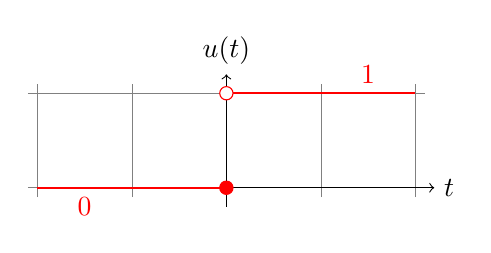
\begin{tikzpicture}[domain=-2:2, scale=1.2]
    \draw[very thin,color=gray] (-2.1,-0.1) grid (2.1,1.1);
    \draw[->] (-2,0) -- (2.2,0) node[right] {$t$};
    \draw[->] (0,-0.2) -- (0,1.2) node[above] {$u(t)$};

    \draw[red,thick] (-2,0) -- (0,0);
    \draw[red,thick] (0,1) -- (2,1);
    \draw[red,fill=white] (0,1) circle (2pt); % Open circle
    \draw[red,fill=red] (0,0) circle (2pt);   % Filled circle

    \node[red] at (1.5, 1.2) {1};
    \node[red] at (-1.5, -0.2) {0};
\end{tikzpicture}

\vspace{1cm}

% Definition for f(t) = g(t)u(t-a)
Now consider the case where $f(t) = g(t)u(t-a)$, where $u(t-a)$ is the shifted unit step function. The Laplace transform of $f(t)$ is:
\[
F(s) = e^{-as} + \mathcal{L}\{g(t-a)\}.
\]

% TikZ diagram for f(t) = g(t)u(t-a)
% \begin{tikzpicture}[domain=-2:4, scale=1.2]
%     \draw[very thin,color=gray] (-2.1,-0.1) grid (4.1,1.1);
%     \draw[->] (-2,0) -- (4.2,0) node[right] {$t$};
%     \draw[->] (0,-0.2) -- (0,1.2) node[above] {$f(t)$};

%     % Step function u(t-a), with g(t) = 1 for simplicity
%     \draw[red,thick] (-2,0) -- (1,0);
%     \draw[red,thick] (1,1) -- (4,1);
%     \draw[red,fill=white] (1,1) circle (2pt); % Open circle
%     \draw[red,fill=red] (1,0) circle (2pt);   % Filled circle

%     \node[red] at (2.5, 1.2) {$g(t)$};
%     \node[red] at (-1.5, -0.2) {0};
%     \node[red] at (1, -0.3) {$t=a$};
% \end{tikzpicture}

The steps to evaluate this are as follows:
\begin{enumerate}
    \item Identify $g(t)$ and $a$
    \item Replace $t$ with $t-a$ to get $g(t-a)$.
    \item Expand $g(t-a)$
    \item Take the Laplace transform. That is, $\Laplace\{g(t-a)\}$
    \item $F(s) = e^{-as}\Laplace\{g(t-a)\}$
\end{enumerate}
\begin{example}
    Evaluate $f(t) = u(t-2)$.


    Note that $g(t) = 1$, and $a=2$. Then, $g(t-2) = 1$. We get $\Laplace\{1\} = \frac{1}{s}$, or $F(s) = e^{-2s}\frac{1}{s}$.
\end{example}

\begin{example}
    Evaluate $f(t) = t^2u(t-2)$.


    Note that $g(t) = t^2$, and $a=2$. Then, $g(t-2) = (t-2)^2$.
    Evaluating, $g(t-2) = t^2-4t+4$. So, Taking the Laplace Transform, we have $\Laplace\{t^2-4t+4\} = \frac{2}{s^3} - \frac{4}{s^2} + \frac{4}{s}$, or $F(s) = e^{-2s}[\frac{2}{s^3} - \frac{4}{s^2} + \frac{4}{s}]$.
\end{example}

\begin{example}
    Evaluate $f(t) = 2 - 3u(t-2) + u(t-3)$.

    We get $F(s) = 2(\frac{1}{s}) - 3 \frac{e^{-2s}}{s} + \frac{e^{-3s}}{s}$.
\end{example}

\begin{example}
    Evaluate $f(t) = 4\cos{t}u(t - \pi)$.

    Recall that $\cos{t-\pi} = -\cos{t}$. This will help us a lot in the future.
    
    Now, we have $a = \pi$, $g(t) = 4\cos{t}$. Then, $g(t-\pi) = 4\cos(t-\pi) = -4\cos{t}$.
    Knowing that $\Laplace\{-4\cos{t}\} = \frac{4s}{s^2+1}$, we get $F(s) = -e^{-\pi s}\frac{4s}{s^2+1}$.
\end{example}

\begin{example}
    Evaluate for $Y(s)$: $y' + y = 4 \cos{t}u(t-\pi)$, given initial conditions $y(0) = 0$.
    \[sY - 0  + Y = e^{-\pi s}\frac{4s}{s^2+1}\]
    \[Y(s+1) = -e^{-\pi s}\frac{4s}{s^2+1} \]
    \[Y(s) = \frac{-e^{-\pi s}\frac{4s}{s^2+1}}{s+1} \]  
\end{example}
But how do we find $Y(t)$? We use the \textit{Second Translation Theorem}.

\begin{defn}
    The \textbf{Second Translation Theorem} in Laplace Transforms is as follows:

    If
    \[
    \mathcal{L}\{f(t)\} = F(s),
    \]
    then
    \[
    \mathcal{L}\{f(t-a)u(t-a)\} = e^{-as}F(s),
    \]
    where $u(t-a)$ is the unit step function that shifts the function by $a$ units in time.
\end{defn}

    % TikZ diagram sketch for the time-shifted function
    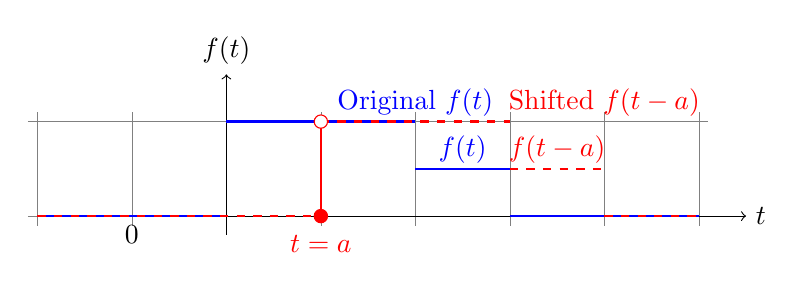
\begin{tikzpicture}[domain=-2:5, scale=1.2]
        \draw[very thin,color=gray] (-2.1,-0.1) grid (5.1,1.1);
        \draw[->] (-2,0) -- (5.5,0) node[right] {$t$};
        \draw[->] (0,-0.2) -- (0,1.5) node[above] {$f(t)$};
    
        % Original function f(t)
        \draw[blue,thick] (-2,0) -- (0,0);
        \draw[blue,thick] (0,1) -- (2,1);
        \draw[blue,thick] (2,0.5) -- (3,0.5);
        \draw[blue,thick] (3,0) -- (5,0);
        \node[blue] at (2.5, 0.7) {$f(t)$};
    
        % Shifted function f(t-a)
        \draw[red,thick, dashed] (-2,0) -- (1,0);
        \draw[red,thick, dashed] (1,1) -- (3,1);
        \draw[red,thick, dashed] (3,0.5) -- (4,0.5);
        \draw[red,thick, dashed] (4,0) -- (5,0);
        \node[red] at (3.5, 0.7) {$f(t-a)$};
    
        % Step at t = a
        \draw[red,thick] (1,0) -- (1,1);
        \draw[red,fill=red] (1,0) circle (2pt);   % Filled circle
        \draw[red,fill=white] (1,1) circle (2pt); % Open circle
        \node[red] at (1, -0.3) {$t = a$};
    
        % Labels
        \node[blue] at (2, 1.2) {Original $f(t)$};
        \node[red] at (4, 1.2) {Shifted $f(t-a)$};
        \node at (-1, -0.2) {0};
    \end{tikzpicture}

    \begin{example}
        $f(t) = (t-1)u(t-1)$. Find $F(s)$. 
        Through some standard malarkey, $F(s) = e^{-s}\frac{1}{s^2}$.
    \end{example}

    \begin{example}
        $F(s) = e^{-2s}\frac{1}{s^3}
    \end{example}
\end{document}
